\begin{figure}
	\centering
	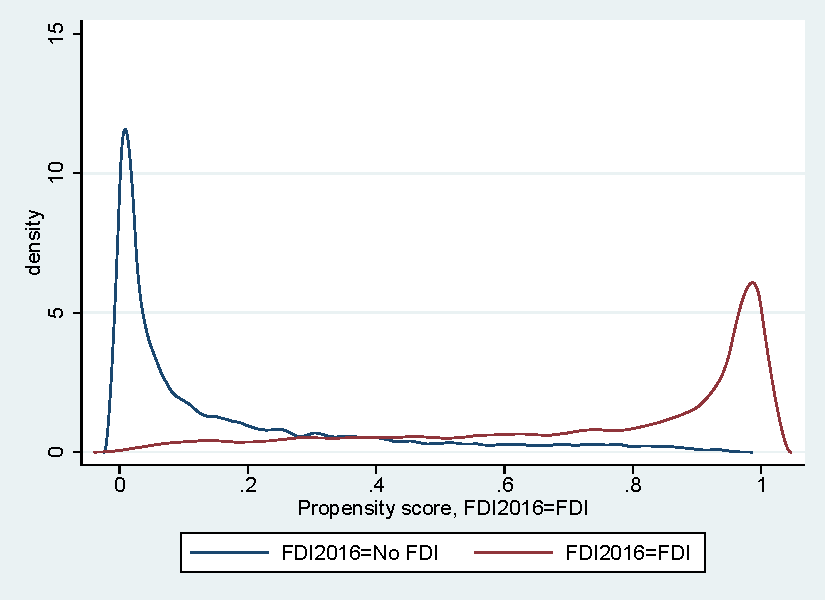
\includegraphics[scale=0.6]{figures_and_tables/3_overlap_intlogit1o1.pdf}\
	\caption{Overlap resulting from the propensity scoring using a logit model (interactions between the set of continuous variables and the set of categorical/binary variables)}
	\label{ol_intlog1}
\end{figure}

\begin{figure}
	\centering
	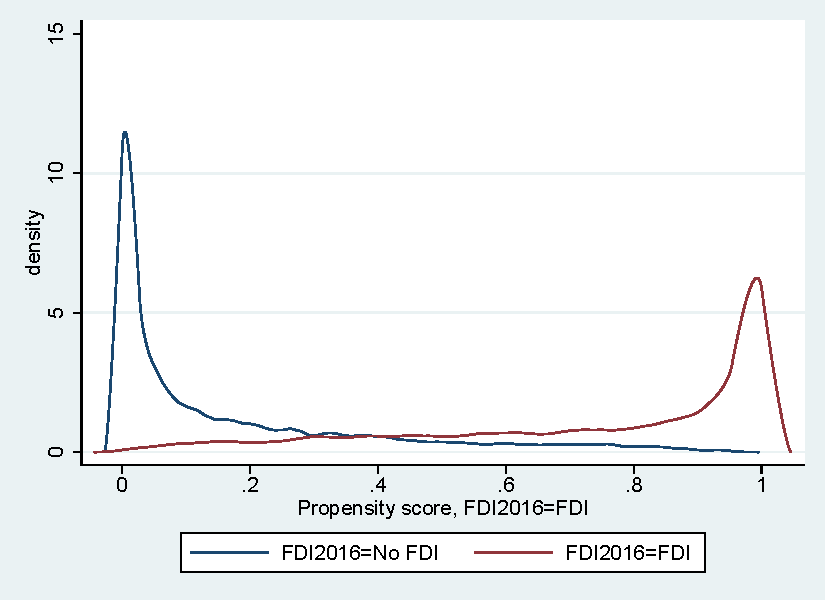
\includegraphics[scale=0.6]{figures_and_tables/3_overlap_intprobit1o1.pdf}\
	\caption{Overlap resulting from the propensity scoring using a probit model (interactions between the set of continuous variables and the set of categorical/binary variables)}
	\label{ol_intprob1}
\end{figure}

\begin{figure}
	\centering
	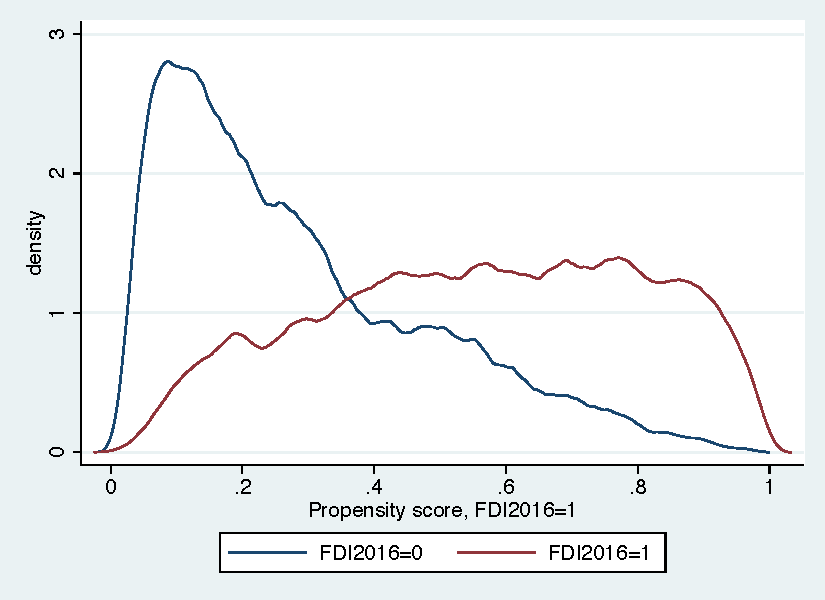
\includegraphics[scale=0.6]{figures_and_tables/3_overlap_linearlogit1o1_reduced.pdf}\
	\caption{Overlap resulting from the propensity scoring using a logit model (linear inclusion of continuous variables only)}
	\label{ol_linlog1_red}
\end{figure}

\begin{table}
	\begin{tabular}{lcccc}
		 \hline \hline
	            &    r(table)&            &            &            \\
            &    Diff:Raw&  Diff:Match&   Ratio:Raw& Ratio:Match\\
0b.RD2015#c.logwages2015&   -.1195646&    .0533576&     .947075&    1.083427\\
1.RD2015#c.logwages2015&    .0055913&    .0622468&    .9912599&    1.316477\\
1b.TECH#c.logwages2015&    .4099088&    .0368431&    1.446385&    1.028314\\
2.TECH#c.logwages2015&    .0985765&    .0250057&    1.221177&    1.058754\\
3.TECH#c.logwages2015&   -.1947846&   -.0206775&    .7998561&    1.052487\\
1b.OWN#c.logwages2015&   -.2416651&   -.0436965&    .3646025&     .827438\\
2.OWN#c.logwages2015&   -.0501523&    -.073387&    .8787442&    .8821358\\
3.OWN#c.logwages2015&    .0095374&    .0913069&    .9615021&    1.220857\\
0b.PORT#c.logwages2015&   -.3780525&    .1312182&    .9245549&    1.171242\\
1b.EXP2015\_CAT#c.logwages2015&   -.4723787&    .1005806&    1.179189&    1.120247\\
0b.RD2015#c.TFP2015&   -.1739665&    .0116561&    .9100893&    1.012206\\
1.RD2015#c.TFP2015&    .0080044&    .0449328&    .9791256&    1.146995\\
1b.TECH#c.TFP2015&    .3830039&    .0380806&    1.517568&    1.029373\\
2.TECH#c.TFP2015&    .0592069&    .0059181&     1.09476&    .9937183\\
3.TECH#c.TFP2015&   -.2626395&   -.0239952&    .6142341&    1.017338\\
1b.OWN#c.TFP2015&   -.2670312&   -.0545362&    .2665297&    .7563862\\
2.OWN#c.TFP2015&    -.064156&   -.0591638&    .8276227&    .8711978\\
3.OWN#c.TFP2015&   -.0408866&    .0506196&    .8831729&    1.080465\\
0b.PORT#c.TFP2015&   -.4416219&    .0664575&    .7259598&     .989018\\
1b.EXP2015\_CAT#c.TFP2015&   -.4566127&    .0384141&    .9833249&    .9922028\\
0b.RD2015#c.logemp2015&    .4513985&    .1458985&    1.015839&    .8251611\\
1.RD2015#c.logemp2015&    .1258157&    .0770499&    1.551717&    1.230311\\
1b.TECH#c.logemp2015&    .4601552&    .0557388&    1.534047&    1.003494\\
2.TECH#c.logemp2015&    .2274026&    .0438903&    1.926955&    1.024059\\
3.TECH#c.logemp2015&    .0899055&   -.0193275&    1.370232&    .8302818\\
1b.OWN#c.logemp2015&   -.0820011&    .0187964&    .9009638&    1.111048\\
2.OWN#c.logemp2015&    .1399032&   -.0080772&    1.482211&    1.009055\\
3.OWN#c.logemp2015&    .2656301&    .1355491&    1.407778&    1.151253\\
0b.PORT#c.logemp2015&    .1339363&    .2636523&     1.28113&    1.094793\\
1b.EXP2015\_CAT#c.logemp2015&    .0840549&    .2223448&    1.142787&    .9004376\\
0b.RD2015#c.DEBTS2015&   -.0687846&    .0529298&    1.018707&    .9896502\\
1.RD2015#c.DEBTS2015&    .0328123&    .0247653&    1.167688&    1.089759\\
1b.TECH#c.DEBTS2015&    .3620529&    .0286521&    1.493647&    1.017304\\
2.TECH#c.DEBTS2015&    .0875624&    .0298535&    1.216558&    1.069462\\
3.TECH#c.DEBTS2015&   -.1987245&   -.0287849&    .7404538&    .9846953\\
1b.OWN#c.DEBTS2015&   -.2451112&   -.0661205&    .3194455&    .6951376\\
2.OWN#c.DEBTS2015&   -.0444712&   -.0452431&    .8861299&    .9559771\\
3.OWN#c.DEBTS2015&   -.0148901&    .0841772&    .9654587&    1.139031\\
0b.PORT#c.DEBTS2015&   -.3147821&    .1120791&    .9126556&    1.079805\\
1b.EXP2015\_CAT#c.DEBTS2015&   -.3607874&    .0860133&    1.078069&    1.028403\\

	 \hline \hline
	\end{tabular}
	\caption{Balance check of the propensity scoring using a logit model (interactions between the set of continuous variables excluding exports and the set of categorical/binary variables including exports) and a 2 on 1 matching procedure}
	\label{bal_intcatlog2}
\end{table}

\begin{table}
	\begin{tabular}{lcccc}
		 \hline \hline
	            &    r(table)&            &            &            \\
            &    Diff:Raw&  Diff:Match&   Ratio:Raw& Ratio:Match\\
0b.RD2015#c.logwages2015&   -.1195646&    .0512606&     .947075&    1.061216\\
1.RD2015#c.logwages2015&    .0055913&    .0554608&    .9912599&    1.266693\\
1b.TECH#c.logwages2015&    .4099088&    .0453662&    1.446385&    1.037856\\
2.TECH#c.logwages2015&    .0985765&     .011763&    1.221177&    1.008307\\
3.TECH#c.logwages2015&   -.1947846&   -.0112131&    .7998561&    1.071675\\
1b.OWN#c.logwages2015&   -.2416651&     -.00517&    .3646025&    .9595119\\
2.OWN#c.logwages2015&   -.0501523&   -.0700267&    .8787442&    .8936324\\
3.OWN#c.logwages2015&    .0095374&    .0653864&    .9615021&    1.159856\\
0b.PORT#c.logwages2015&   -.3780525&     .120801&    .9245549&    1.140006\\
1b.EXP2015\_CAT#c.logwages2015&   -.4723787&    .0957885&    1.179189&    1.085749\\
0b.RD2015#c.TFP2015&   -.1739665&   -.0176556&    .9100893&    .9616481\\
1.RD2015#c.TFP2015&    .0080044&    .0449186&    .9791256&    1.144561\\
1b.TECH#c.TFP2015&    .3830039&    .0394225&    1.517568&    1.019847\\
2.TECH#c.TFP2015&    .0592069&    .0021288&     1.09476&    .9735207\\
3.TECH#c.TFP2015&   -.2626395&   -.0295988&    .6142341&    .9941437\\
1b.OWN#c.TFP2015&   -.2670312&   -.0223185&    .2665297&    .8203311\\
2.OWN#c.TFP2015&    -.064156&   -.0677646&    .8276227&    .8347698\\
3.OWN#c.TFP2015&   -.0408866&    .0193216&    .8831729&    1.021586\\
0b.PORT#c.TFP2015&   -.4416219&     .041847&    .7259598&    .9348855\\
1b.EXP2015\_CAT#c.TFP2015&   -.4566127&    .0159171&    .9833249&    .9485514\\
0b.RD2015#c.logemp2015&    .4513985&    .1416871&    1.015839&    .8061887\\
1.RD2015#c.logemp2015&    .1258157&     .078879&    1.551717&    1.246292\\
1b.TECH#c.logemp2015&    .4601552&    .0592596&    1.534047&     1.00785\\
2.TECH#c.logemp2015&    .2274026&    .0425132&    1.926955&    1.032892\\
3.TECH#c.logemp2015&    .0899055&   -.0237793&    1.370232&    .8161867\\
1b.OWN#c.logemp2015&   -.0820011&    .0683805&    .9009638&    1.402103\\
2.OWN#c.logemp2015&    .1399032&   -.0186314&    1.482211&    .9648858\\
3.OWN#c.logemp2015&    .2656301&    .1108782&    1.407778&    1.093449\\
0b.PORT#c.logemp2015&    .1339363&    .2622673&     1.28113&    1.085431\\
1b.EXP2015\_CAT#c.logemp2015&    .0840549&    .2246056&    1.142787&    .8873473\\
0b.RD2015#c.DEBTS2015&   -.0687846&    .0601309&    1.018707&     1.00674\\
1.RD2015#c.DEBTS2015&    .0328123&    .0212035&    1.167688&    1.081422\\
1b.TECH#c.DEBTS2015&    .3620529&    .0308845&    1.493647&    1.013492\\
2.TECH#c.DEBTS2015&    .0875624&    .0220798&    1.216558&    1.041233\\
3.TECH#c.DEBTS2015&   -.1987245&   -.0172314&    .7404538&    1.008782\\
1b.OWN#c.DEBTS2015&   -.2451112&   -.0274972&    .3194455&    .8041278\\
2.OWN#c.DEBTS2015&   -.0444712&    -.047437&    .8861299&    .9560576\\
3.OWN#c.DEBTS2015&   -.0148901&    .0678248&    .9654587&    1.114978\\
0b.PORT#c.DEBTS2015&   -.3147821&    .1155958&    .9126556&    1.103188\\
1b.EXP2015\_CAT#c.DEBTS2015&   -.3607874&    .0898824&    1.078069&    1.043331\\

	 \hline \hline
	\end{tabular}
	\caption{Balance check of the propensity scoring using a logit model (interactions between the set of continuous variables excluding exports and the set of categorical/binary variables including exports) and a 4 on 1 matching procedure}
	\label{bal_intcatlog4}
\end{table}

\begin{table}
	\begin{tabular}{lcccc}
		 \hline \hline
		            &    r(table)&            &            &            \\
            &    Diff:Raw&  Diff:Match&   Ratio:Raw& Ratio:Match\\
0b.RD2015#c.logwages2015&   -.1195646&    .0075964&     .947075&    1.111949\\
1.RD2015#c.logwages2015&    .0055913&    .0678727&    .9912599&     1.29589\\
1b.TECH#c.logwages2015&    .4099088&    .0882317&    1.446385&     1.06342\\
2.TECH#c.logwages2015&    .0985765&    .0323807&    1.221177&    1.063771\\
3.TECH#c.logwages2015&   -.1947846&   -.1157132&    .7998561&     .979123\\
1b.OWN#c.logwages2015&   -.2416651&   -.0474861&    .3646025&      .81565\\
2.OWN#c.logwages2015&   -.0501523&   -.0520133&    .8787442&    .9046346\\
3.OWN#c.logwages2015&    .0095374&    .0802055&    .9615021&    1.167214\\
0b.PORT#c.logwages2015&   -.3780525&    .1182721&    .9245549&    1.138085\\
1b.EXP2015\_CAT#c.logwages2015&   -.4723787&    .1161452&    1.179189&    1.043137\\
0b.RD2015#c.TFP2015&   -.1739665&    .0042368&    .9100893&    .9940214\\
1.RD2015#c.TFP2015&    .0080044&    .0585258&    .9791256&     1.20869\\
1b.TECH#c.TFP2015&    .3830039&    .0836885&    1.517568&    1.071151\\
2.TECH#c.TFP2015&    .0592069&    .0318663&     1.09476&    1.067882\\
3.TECH#c.TFP2015&   -.2626395&   -.0953681&    .6142341&    .9447969\\
1b.OWN#c.TFP2015&   -.2670312&   -.0664198&    .2665297&    .6787129\\
2.OWN#c.TFP2015&    -.064156&   -.0446857&    .8276227&    .8718027\\
3.OWN#c.TFP2015&   -.0408866&    .0486999&    .8831729&    1.057604\\
0b.PORT#c.TFP2015&   -.4416219&    .0625049&    .7259598&    .9615733\\
1b.EXP2015\_CAT#c.TFP2015&   -.4566127&    .0591635&    .9833249&    .9540943\\
0b.RD2015#c.logemp2015&    .4513985&   -.0328685&    1.015839&    .5844724\\
1.RD2015#c.logemp2015&    .1258157&    .0947427&    1.551717&    1.318069\\
1b.TECH#c.logemp2015&    .4601552&    .0884816&    1.534047&    .9960945\\
2.TECH#c.logemp2015&    .2274026&    .0507278&    1.926955&    1.019688\\
3.TECH#c.logemp2015&    .0899055&   -.2195556&    1.370232&    .4494659\\
1b.OWN#c.logemp2015&   -.0820011&     .030118&    .9009638&    1.240997\\
2.OWN#c.logemp2015&    .1399032&    -.003491&    1.482211&    .9428245\\
3.OWN#c.logemp2015&    .2656301&    .1296749&    1.407778&    1.105473\\
0b.PORT#c.logemp2015&    .1339363&    .2443691&     1.28113&    1.037298\\
1b.EXP2015\_CAT#c.logemp2015&    .0840549&    .2410722&    1.142787&    .8458924\\
0b.RD2015#c.DEBTS2015&   -.0687846&   -.0252322&    1.018707&    .9472902\\
1.RD2015#c.DEBTS2015&    .0328123&    .0394126&    1.167688&    1.141701\\
1b.TECH#c.DEBTS2015&    .3620529&    .0882979&    1.493647&    1.077583\\
2.TECH#c.DEBTS2015&    .0875624&    .0364184&    1.216558&     1.08119\\
3.TECH#c.DEBTS2015&   -.1987245&   -.1889552&    .7404538&    .7389029\\
1b.OWN#c.DEBTS2015&   -.2451112&   -.0669317&    .3194455&    .6746464\\
2.OWN#c.DEBTS2015&   -.0444712&   -.0128759&    .8861299&     1.01678\\
3.OWN#c.DEBTS2015&   -.0148901&     .071986&    .9654587&    1.111722\\
0b.PORT#c.DEBTS2015&   -.3147821&      .12112&    .9126556&    1.099798\\
1b.EXP2015\_CAT#c.DEBTS2015&   -.3607874&    .1209194&    1.078069&    1.019338\\

		 \hline \hline
	\end{tabular}
	\caption{Balance check of AIPW estimation (using interactions between the set of continuous variables excluding exports and the set of categorical/binary variables including exports)} 
	\label{bal_aipw}
\end{table}
